\chapter{Elección de herramientas}

\section{Elección de una herramienta base}
En la búsqueda de una herramienta para la detección del plagio encontré diversos servicios como Viper \cite{viper}, Grammarly \cite{grammarly}, Ithenticate \cite{ithenticate}, Plagscan \cite{plagscan} y Turnitin. Entre ellos destaca este último dado que cuenta con una gran base de datos con contenido web, artículos previamente enviados y publicaciones \cite{turnitin}.
\newline
El acceso a estos servicios se hace a través de su interfaz web y está limitado a universidades y otras instituciones o es necesario tener un plan de suscripción de pago.
\newline
Estas herramientas no detectan plagio en sí, sino que devuelven un índice de similaridad entre los archivos enviados y el resto de archivos que tienen en su base de datos.
\newline
Esta similaridad la calculan comparando parámetros como la frecuencia de uso de cada palabra, el parafraseo o la copia literal \cite{plagio_estrategias}.
\newline
Estas herramientas fueron creadas para detectar plagio en trabajos de alumnos escritos en texto plano tales como artículos o memorias de proyectos.
\newline
Es por todo esto que estos servicios no son los más indicados para detectar plagio en archivos de código, a menos que se quiera comprobar si el alumno se ha copiado palabra a palabra de algún archivo de código encontrado online.

\bigskip

Se buscaron por tanto herramientas para la detección de plagio en programas en código fuente.
Existen numerosas herramientas que cumplen ese propósito. En la tabla de la Figura \ref{fig:figura1} muestro las más usadas aunque también debo mencionar: Sherlock \cite{sherlock}, GPlag \cite{gplag}, Marble, Holmes \cite{Moss_Jplag_info} y YAP3 \cite{yap3}. 
\newline
Estos sistemas de detección tienden a adoptar métricas basadas en diferentes aspectos de un archivo de código tales como la complejidad de los flujos de control que se están usando, el número de estructuras de datos que hay de cada tipo, los nombres de las variables y la cantidad de comentarios \cite{plagio_estrategias}.
\newline
Las herramientas que mejores resultados ofrecen y generalmente usan los colegios, universidades, academias y otras instituciones para la detección de plagio entre sus alumnos son MOSS y JPLAG.
\newline
\bigskip
A continuación se explica en qué consiste cada una de estas.


\section{MOSS}

MOSS (Measure Of Software Similarity) es un sistema automático para determinar la similaridad entre programas \cite{Moss_web}, desarrollado en 1994 por Alex Aiken \cite{Moss_uso}, profesor en UC Berlekey en aquel entonces.
\newline
MOSS está disponible como servicio web mediante un servidor que recibe las peticiones que se le envíen a partir de un script en Perl (facilitado por correo automáticamente si lo solicitas). El servidor procesa los archivos enviados con las opciones que se le especifica y devuelve los resultados a través de una interfaz web (devuelve un enlace a los resultados).
\newline
Para proteger la confidencialidad del código de los archivos que se envían al servidor, los resultados generados analizando tal código se borran del servidor 14 días después de su envío.
\newline
Para enviar una petición al servidor tan solo se tendrá que llamar al script usando una opción de comandos similar a la siguiente (partiendo de que el script y los archivos se encuentran en el directorio actual):

\bigskip
\begin{center}
 moss -l matlab *.m
\end{center}
\bigskip

Existen diversas opciones más que podemos usar además de -l. En el primera apartado del capítulo ''Ejecución y Pruebas'' se explican en más detalle.  
\newline
En el siguiente subapartado explicamos en qué consiste su algoritmo de detección.

\subsection{Algoritmo usado}

MOSS se basa en usar n-gramas a nivel de carácter como criterio de comparación entre archivos \cite{Moss_algoritmo}, esta es una ténica comunmente usada en herramientas de detección de plagio. Un n-grama es una subcadena contigua de n elementos, por ejemplo, con n = 5, si tenemos la siguiente cadena en un documento:

\begin{center}
abbcadarrad
\end{center}

Los 5-gramas que se obtienen de esta serán:

\begin{center}
abbca  bbcad  bcada  cadar  adarr  darra  arrad
\end{center}

Una vez obtenidos los n-gramas del documento completo, se le calcula a cada uno un identificador propio (hash) basado en la localización del n-grama en el documento y en los carácteres que lo componen.
\newline
A continuación, se elige un subconjunto de estos hashes para representar al documento (no podemos coger todos los hashes por motivos de eficiencia ya que habrá casi tantos hashes como carácteres en el archivo).
\newline
De esta forma, si la funcion resumen (hash) usada tiene una probabilidad de colisiones pequeña (una colisión consiste en que dos cadenas diferentes tengan la misma función resumen) cuando dos documentos tengan en común algún hash será extremadamente probable que también compartan n-gramas, esto es lo que usa MOSS para calcular similaridad entre programas.
\newline
Para determinar qué funciones resumen escoger normalmente se usa la estrategia de elegir las que sean 0 mod p, para algún p fijo. Esta estrategia es fácil de implementar y nos quedamos únicamente con 1/p de todos los hashes para representar el documento.
\newline
Este método no garantiza que se detecten similaridades entre archivos ya que sólo se detectarán n-gramas iguales cuyo hash sea 0 mod p.
\newline
MOSS soluciona este problema con una técnica llamada windowing (procesar por ventanas).
\newline
En lugar de seleccionar n-gramas aleatorios MOSS selecciona como mínimo una función resumen por cada ventana de un cierto tamaño previamente establecido. Además MOSS usa un valor de n (longitud de n-gramas) grande para evitar ruido en los resultados \cite{Moss_Jplag_info}.

\subsection{Ejemplo de ejecución}
MOSS devuelve los resultados en un enlace que nos lleva a una página con los índices de similaridad entre los archivos enviados tal y como podemos ver en la figura \ref{fig:ej_MOSS1}.
\newline
Si pinchamos en el nombre de algún archivo de los comparados visualizaremos una página en la que se comparan los dos códigos lado a lado como podemos ver en figura \ref{fig:ej_MOSS2}.
En el capítulo de Ejecución y Pruebas se explica con mayor detalle como interpretar estos resultados.

\begin{figure}[H] %con el [H] le obligamos a situar aquí la figura
\centering
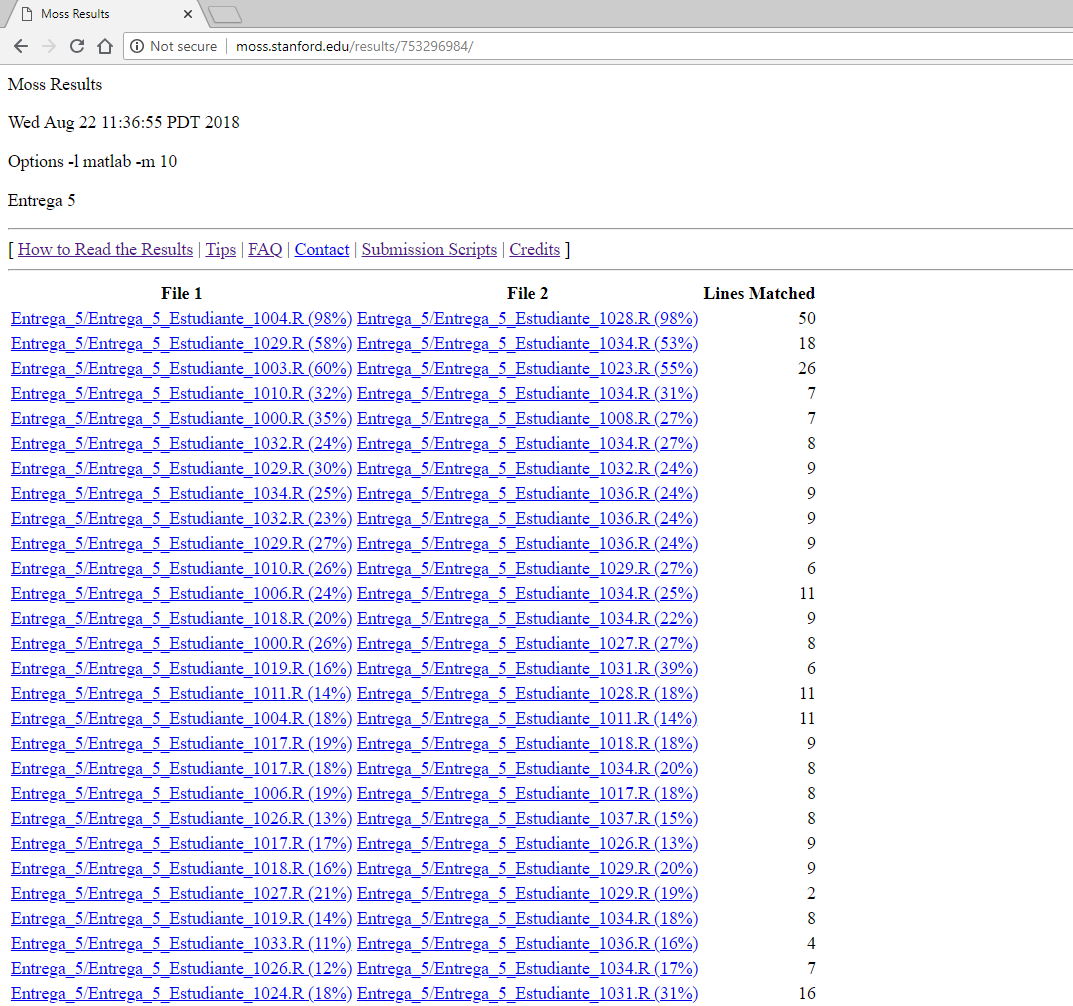
\includegraphics[ width=13cm, height=15cm]{imagenes/MOSS_ejemplo_inicial.png}  %el parámetro scale permite agrandar o achicar la imagen. En el nombre de archivo puede especificar directorios
\caption{Ejemplo de página principal de resultados (MOSS) } \label{fig:ej_MOSS1}
\end{figure}

\begin{figure}[H] %con el [H] le obligamos a situar aquí la figura
\centering
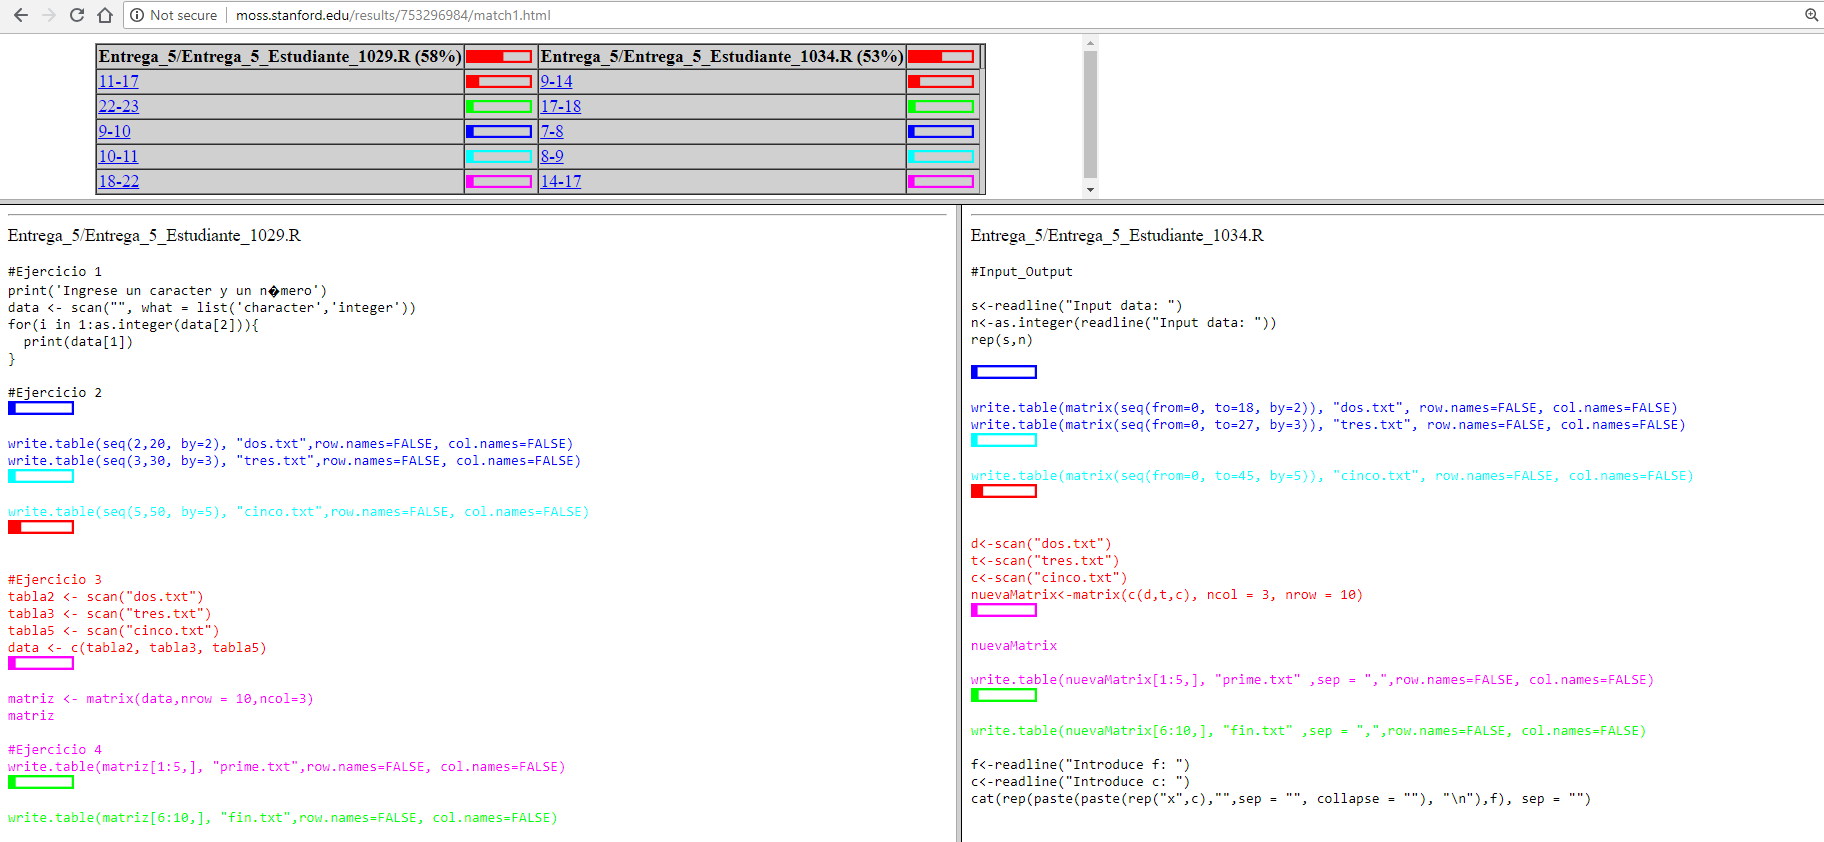
\includegraphics[ height=11cm, width=13cm]{imagenes/MOSS_ejemplo_comparacion.png}  %el parámetro scale permite agrandar o achicar la imagen. En el nombre de archivo puede especificar directorios
\caption{Ejemplo de página de comparación de código de MOSS} \label{fig:ej_MOSS2}
\end{figure}

\section{JPLAG}
JPLAG es un sistema que encuentra similaridades entre conjuntos de archivos en código fuente \cite{web_jplag}. Fue desarrollado por Guido Malpohl en 1996. 
\newline
JPLAG fue creado con la idea de que comparar programas basándose en un vector de características no es suficiente, ya que esto ignora gran parte de la similaridad estructural entre programas \cite{Moss_Jplag_info}. Es por esto que en su lugar intenta emparejar a partir de características estructurales convirtiendo primero el código en una lista de tokens para después aplicar un algoritmo que encuentra emparejamientos entre las listas de tokens obtenidas priorizando emparejamientos lo más largos posible.
\newline
Para usar esta herramienta es necesario descargar su código disponible en Github\cite{jplag_github} y ejecutarlo localmente en nuestro PC. JPLAG genera entonces un conjunto de páginas en HTML con los resultados.
\newline
JPLAG también está disponible como servicio web aunque sus propios desarrolladores no recomiendan su uso ya que usa bibliotecas anticuadas y no está acabado (además de que ya no aceptan nuevos registros).

\subsection{Algoritmo usado}

JPLAG opera en 2 fases \cite{jplag_paper}:
\begin{enumerate}
\item Se analizan sintácticamente o léxicamente(dependiendo del lenguaje) todos los programas enviados, convirtiéndolos en cadenas de tokens.
\item Se comparan las cadenas de tokens por pares.
\end{enumerate}


\subsubsection{1. Análisis Sintáctico}
Esta es la única parte que depende del lenguaje en cuestión en el que están escritos los archivos que se envían a JPLAG. Se trata del frontend de JPLAG.
\newline
El frontend se encarga de realizar un análisis sintáctico o léxico (parser o scanner) de los archivos para reconocer los tokens que los componen como podemos apreciar en la figura \ref{fig:ej_JPLAG1}.

\begin{figure}[H] %con el [H] le obligamos a situar aquí la figura
\centering
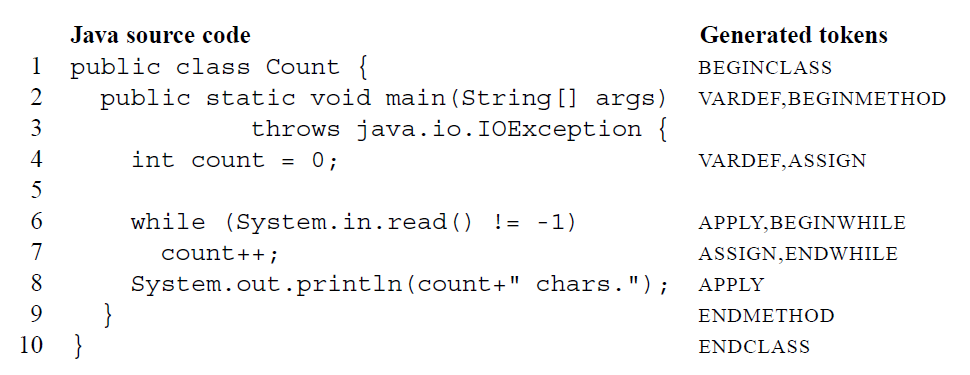
\includegraphics[scale=0.5]{imagenes/JPLAG_ejemplo_tokens.png}  %el parámetro scale permite agrandar o achicar la imagen. En el nombre de archivo puede especificar directorios
\caption{Ejemplo de tokens extraidos de código en java } \label{fig:ej_JPLAG1}
\end{figure}


Los tokens que se escogen deben de ser representativos del lenguaje que estemos tratando para que capturen la esencia del programa (la cual es difícil de cambiar por un plagiador).
\newline
Los espacios en blanco y los comentarios nunca se deben de tener en cuenta como tokens.


\subsubsection{2. Comparación de los tokens}
El algoritmo usado para comparar las cadenas de tokens es básicamente Greedy String Tiling, algoritmo desarrollado por Michael Wise, creador de YAP3, herramienta donde lo aplica \cite{yap3}.
\newline
Cuando se comparan 2 cadenas de tokens deben cumplirse tres reglas:
\begin{enumerate}
\item Un token de una cadena sólo puede ser asociado a un token de la cadena con la que se compara.
\item Las subcadenas de tokens deben de ser independientes de su posición en la cadena principal de tokens. 
\item Tendrán preferencia los emparejamientos largos (de muchos tokens seguidos) sobre los cortos.
\newline
\end{enumerate}

\bigskip
Al aplicar la tercera regla estamos ante un algotimo voraz (greedy) que consiste en tres bucles anidados: el primer bucle itera sobre todos los tokens de la primera cadena (que llamaremos X), el segundo bucle compara el token en el que estamos de X con cada token de la segunda cadena (que llamaremos Y), en caso de ser el mismo token en algún punto del segundo bucle se entra en el tercer bucle, donde se siguen comparando entre X e Y para ver cuántos tokens seguidos son iguales desde ese punto. 
\newline Una vez hecho esto marcamos los emparejamientos de mayor longitud encontrados y repetimos el proceso completo una y otra vez pero sin tener en cuenta en cada vuelta los tokens que ya han sido marcados.
\newline Se repite el proceso hasta que no se encuentre ningún emparejamiento.  

\bigskip
Este es el algoritmo que usa JPLAG con la diferencia de le aplica algunas optimizaciones en tiempo de ejecución. Aunque la complejidad del algoritmo en el peor caso ($\mathcal{O}(n^3)$) no se puede reducir, sí que es posible reducir la complejidad media de los casos prácticos a $\mathcal{O}(n)$.
\newline
Esto es lo que consigue JPLAG adaptando al algoritmo de greedy string tiling la idea del algoritmo de Karp-Rabin \cite{Rabin} en el cual se encuentran ocurrencias de una cadena corta en otra larga usando funciones hash.


\subsection{Ejemplo de ejecución}
JPLAG devuelve los resultados en un conjunto de páginas HTML cuya página principal muestra los mayores índices de similaridad entre los archivos enviados junto con un histograma con todos los índices entre los archivos tal y como podemos ver en la figura \ref{fig:ej_JPLAG2}.
\newline
Si pinchamos en el nombre de algún archivo de los comparados visualizaremos una página en la que se comparan los dos códigos lado a lado como podemos ver en figura \ref{fig:ej_JPLAG3}.
Podemos apreciar que la forma de devolver los resultados de MOSS y JPLAG son muy similares, esto se debe a que la interfaz web de MOSS también la hizo Guido Malpohl(creador de JPLAG) \cite{moss_credits}.

\begin{figure}[H] %con el [H] le obligamos a situar aquí la figura
\centering
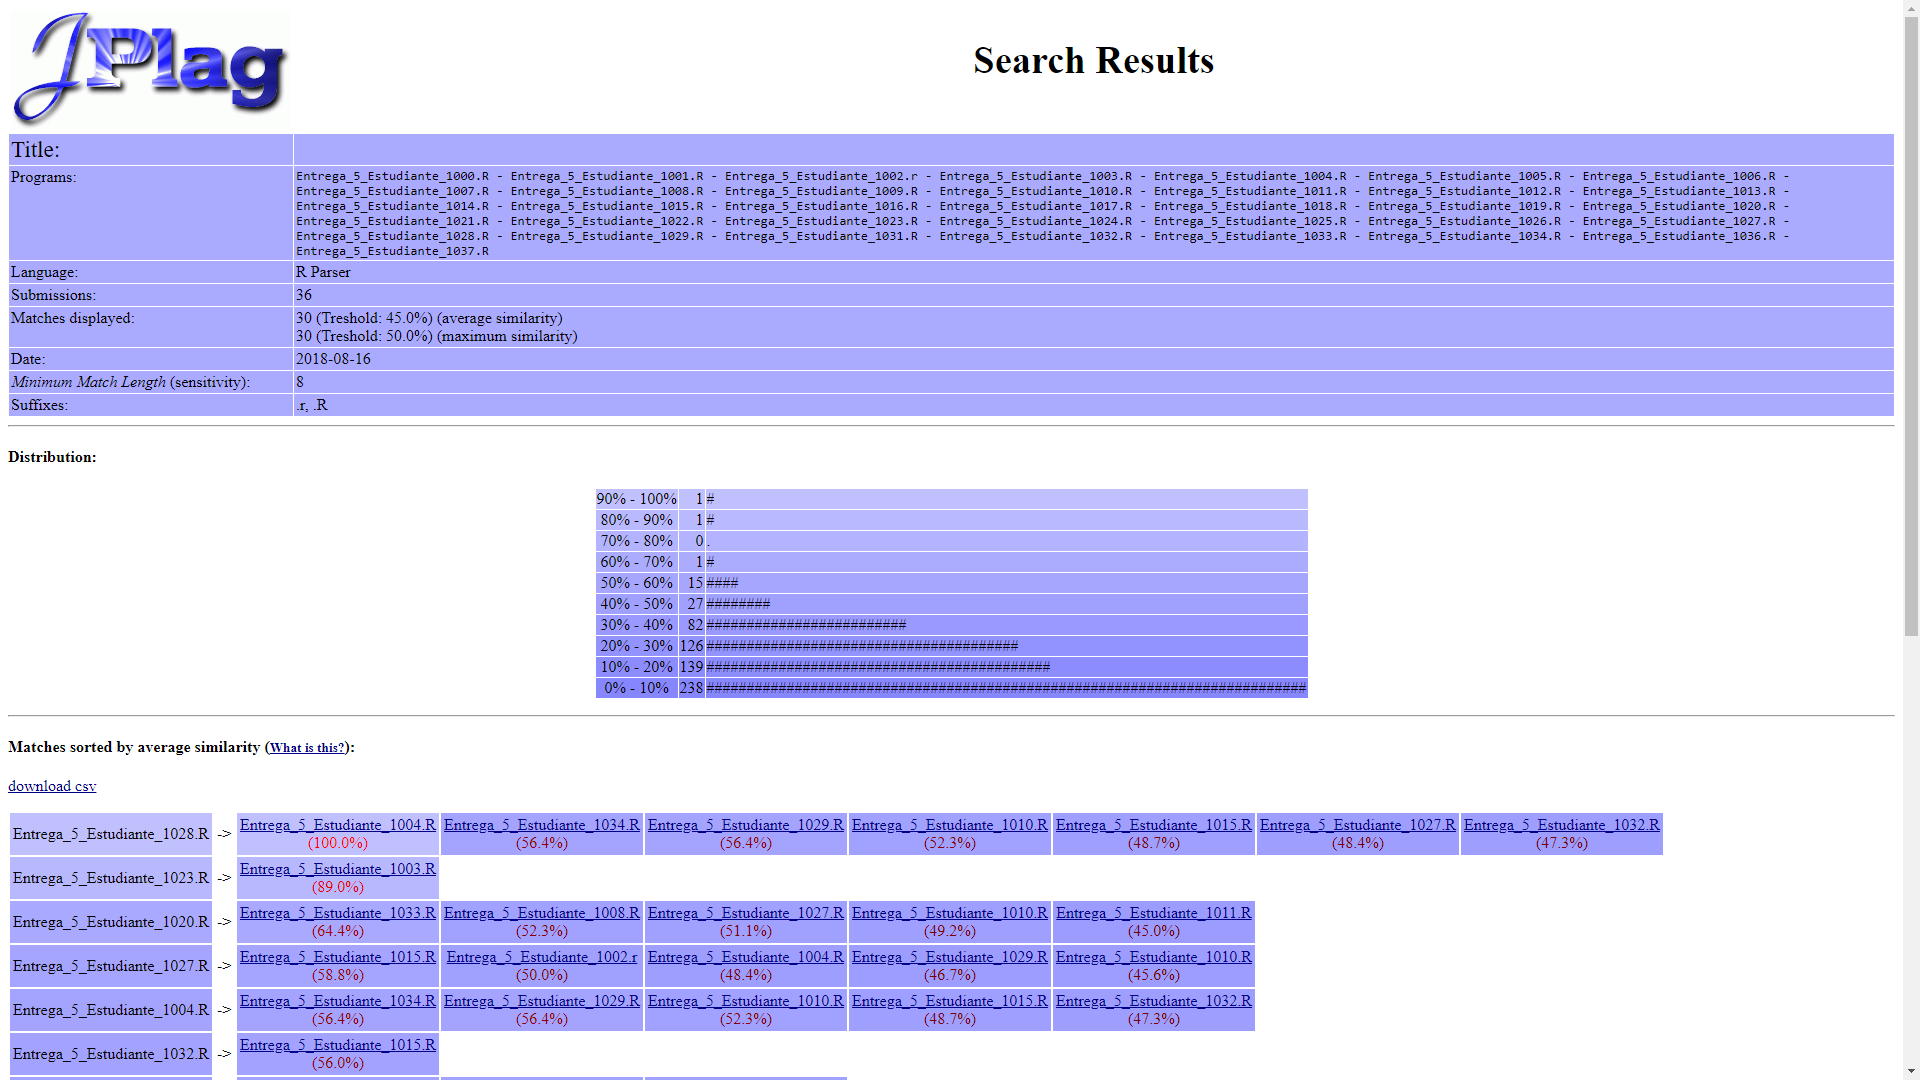
\includegraphics[ width=14cm, height=14cm]{imagenes/JPLAG_ejemplo_inicial.png}  %el parámetro scale permite agrandar o achicar la imagen. En el nombre de archivo puede especificar directorios
\caption{Ejemplo de página principal de resultados (JPLAG) } \label{fig:ej_JPLAG2}
\end{figure}

\begin{figure}[H] %con el [H] le obligamos a situar aquí la figura
\centering
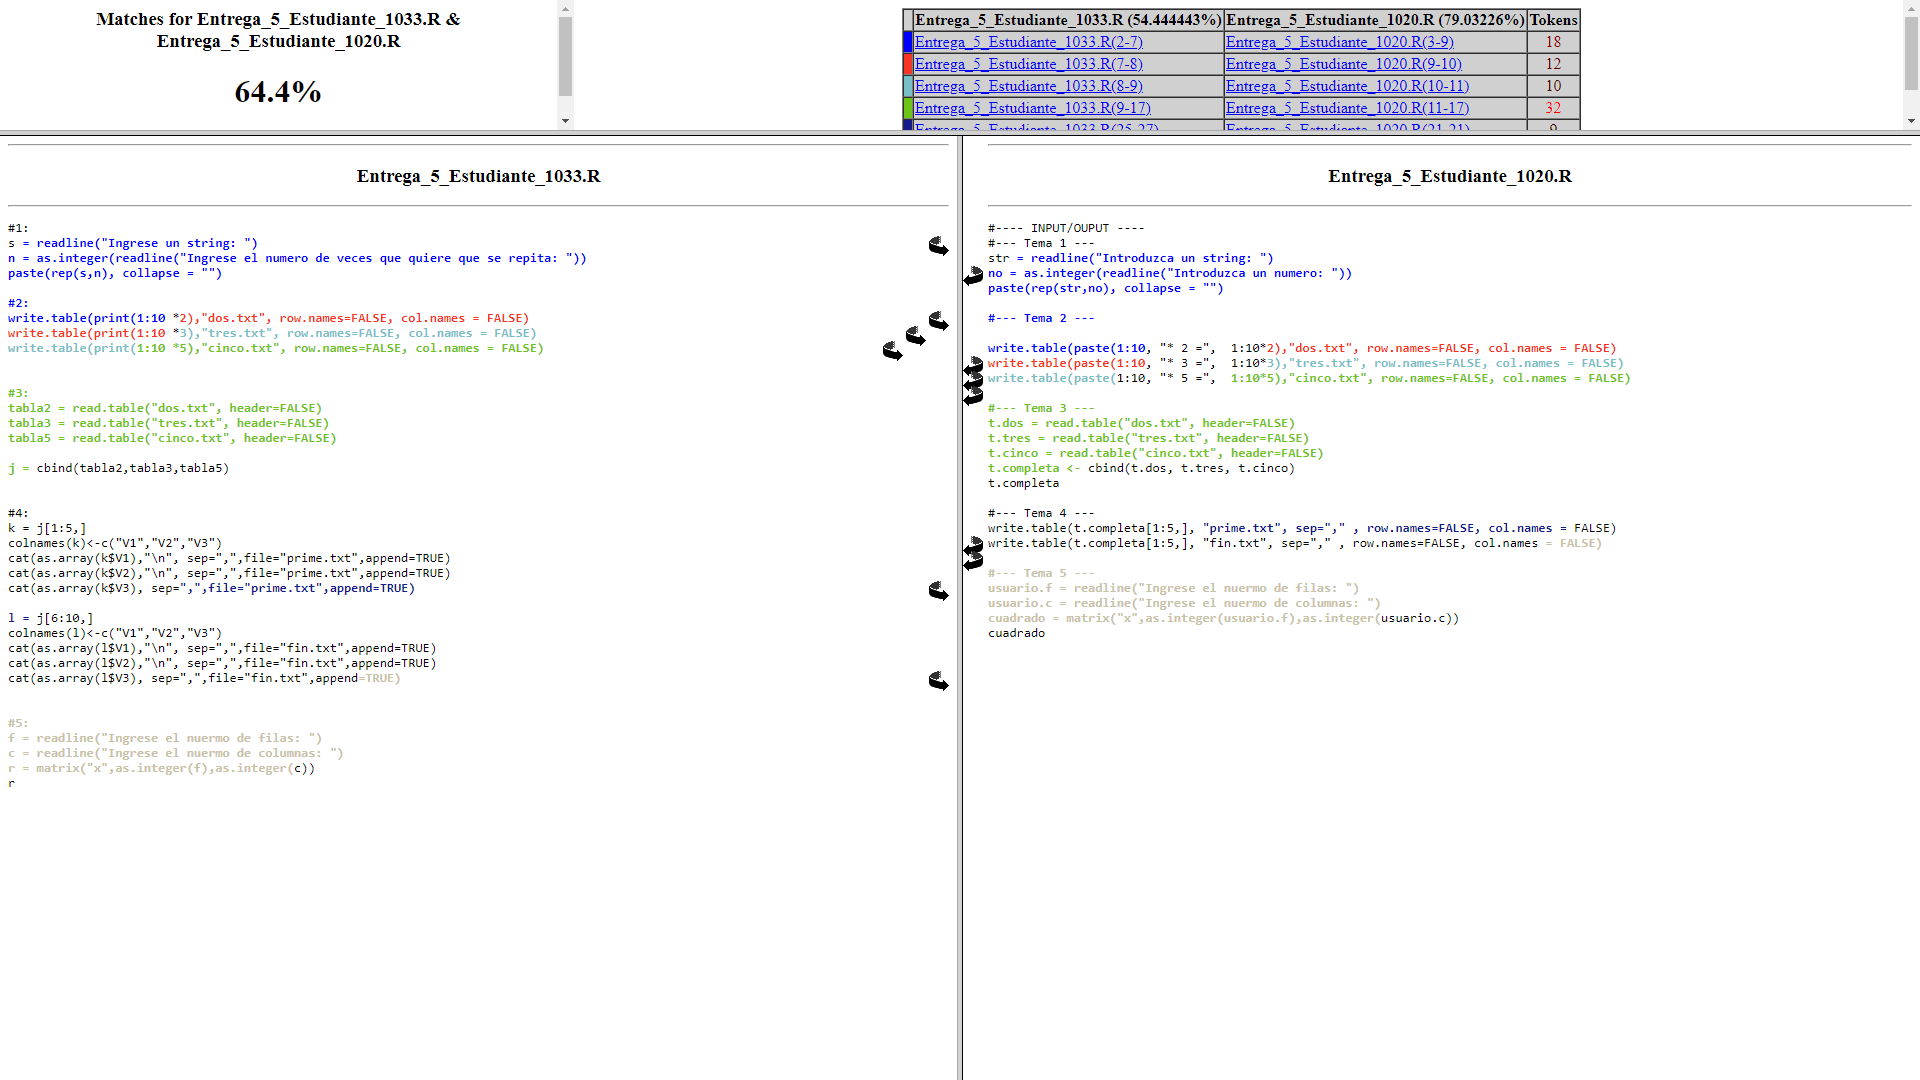
\includegraphics[ height=11cm, width=13cm]{imagenes/JPLAG_ejemplo_comparacion.png}  %el parámetro scale permite agrandar o achicar la imagen. En el nombre de archivo puede especificar directorios
\caption{Ejemplo de página de comparación de código de JPLAG} \label{fig:ej_JPLAG3}
\end{figure}

\subsection{Razones de su elección}
Dado que JPLAG es más fácilmente modificable, debido a que su código está disponible y no es necesario cambiar el algoritmo principal que usa para que funcione con otros lenguajes, (tan solo hay que crear un frontend) JPLAG ha sido la herramienta escogida para adaptar a R.


